\section{Overarching design patterns for \nep}\label{sec:overarchpat}

\subsection{Domain-specific patterns for scientific computing}

This section reflects the state of \nep\ at the time of writing: there are, as
yet, no detailed designs for the proxyapps (this is the division between
specification and development); and as a result, this report is correctly to
be regarded as a living document.
That said, some progress can be made by realizing that the forthcoming
proxyapps form the prototype components for a modular scientific simulation
framework fitting precisely the description of a {\it System for modeling and
simulation} given by Sommerville~\cite{sommerville}:

\begin{quote}
These are systems that are developed by
scientists and engineers to model physical processes or situations, which include
many separate, interacting objects. These are often computationally intensive
and require high-performance parallel systems for execution.
\end{quote}

It is for example clear at this point that the lion's share of the \nep\ code
will be written in object-oriented languages: most of the core proxyapps will
be written in C++ in order to leverage existing componentized frameworks (as
mentioned above, the {\it Nektar++} framework makes extensive use of
object-oriented methods~\cite{Mo20Nekt}).
Accordingly, much of the tried and tested pattern language developed in
\cite{gammahelmjohnsonvlissides} and thereafter is relevant (and, further,
the proxyapps have the potential to benefit from the advantages of the Object
pattern described by Rouson et al in Ch.5 of~\cite{rousonxiaxu}).  
As regards the trade-off between object-oriented coding and ultimate
performance, it might be noted that these frameworks have proven scaling to
at least thousands of processor cores.

Applications of software patterns to scientific computing are yet more
directly germane, if sadly rare: the current edition of \cite{rousonxiaxu}, a
textbook aiming to provide a lexicon of domain-specific design patterns aimed
at multiphysics applications, was published in 2014 and it explicitly
highlights (p.6) the relative paucity of references for design patterns
specific to scientific computing as of that date.
The book culminates in the Morfeus framework, a proposal that seems to have
been aimed at providing an implementation of many of the book's ideas, though
it restricts itself to Fortran.
Some other salient domain-specific patterns are outlined in the article by
Blilie \cite{Bl02Patt}, including, for example, how to handle quantities
with physical units.
Quantities with units raise a number of concerns in scientific programming: a
judicious choice can result in simplification of the code, eliminating
unnecessary floating-point operations (one straightforward example is
removing $\epsilon_0$ and $\mu_0$ when simulating Maxwell's equations, by
rescaling the variables representing the magnetic field and the time), as
well as improving readability; and a consistent overall strategy for units is
obviously required when coupling different proxyapps.
This paper highlights also the fact that design patterns can help in the
division of labour between domain specialists (i.e. physicists) and experienced
software engineers, in that those specialists can use the UML representations
to specify the code structure in a language-independent form, to be
implemented in detail by software developers with little or no domain
expertise.
In addition, \cite{Bl02Patt} outlines two general patterns to be used for
treating the generic types of problem treated by physics software: particles
on one hand and continuous systems (a.k.a fields) on the other, highlighting
that useful simplifications can be made in order to handle multiple timescales
(for example, updating the fast particle dynamics at a higher time resolution
than that of the fields), though a note of caution is sounded if the physics
of the problem is tightly coupled.

\subsection{Architectural patterns}

Architectural design patterns occupy a level just beneath that of the overall
application framework (into which falls the question of division into
libraries and appropriate directory structures) and were first defined by
Garlan and Shaw in 1996 \cite{garlanshaw}, there called {\it architectural
styles}.  
They govern overall program control and coordination.  Given the incremental
development and delivery strategy adopted in \nep, a detailed discussion of
the final architecture (falling under the definition of {\it architecture in
the large} given in ch.6 of Sommerville \cite{sommerville}) is perhaps
premature at this point.  
In future, wisdom in this area could be gleaned by closer study of existing
architectures, for example the United States' {\it One Modeling Framework for
Integrated Tasks} (OMFIT) system \cite{omfitwebsite} and the ITER {\it
Integrated Modelling and Analysis Suite} (IMAS) \cite{Im15Desi}, the latter of
which uses the Kepler scientific workflow system \cite{keplerwebsite}, even
for fine-grained component integration.  
On an individual proxyapp level, called {\it architecture in the small},
application architectures are again determined to an extent by the re-use of
existing frameworks.

One interesting scheme is the layered architectural pattern, which, as well as
giving localization of change, may be used to provide performance portability;
as a topical example, algorithmic content could be implemented in terms of the
API of an abstraction layer such as SYCL \cite{syclwebsite}, Kokkos
\cite{kokkoswebsite} or RAJA \cite{rajawebsite}.  
Although there is a one-off overhead in writing the initial implementation in
terms of the chosen API (though some aim to provide a C++-like programming
experience), the code is thereafter portable between any of the platforms supported
by the abstraction layer, with little additional programmer burden (see
Fig.\ref{fig:sycllayer}).  
These abstraction layers are somewhat new technology at the time of writing
and it is certainly possible to envisage cases in which the performance achieved might
be bettered by a platform-specific implementation (though see
\cite{De20Eval} for an analysis of the relative performance of
SYCL vs. native code for a standard benchmark based on HPC-style
applications).  
This paradigm offers a potential route to a more sustainable code, since the
abstraction layers avoid tying to one platform; moreover, they may also be
extensible to future accelerator types.  
It is also a significant step in the direction of what Rouson et al
\cite{rousonxiaxu} refer to as the holy grail of parallel scalability, to wit
{\it automatic parallelization of code without direct programmer
intervention}.

\begin{figure}
\centerline{\rotatebox{0}{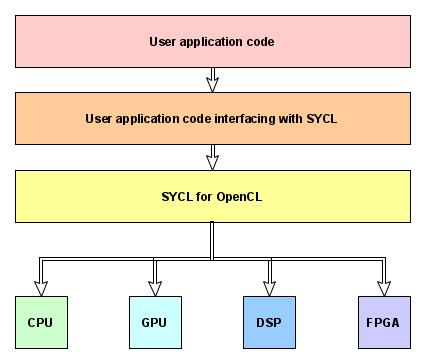
\includegraphics[width=10.5cm]{../png/sycl_layer.jpg}}}
\caption{\label{fig:sycllayer}
Diagram illustrating layered structure of an application using an abstraction layer (SYCL here).  Only the layer directly addressing SYCL would require recompilation to port the code between different accelerator types.}
\end{figure}
\clearpage
\subsection{Concurrency patterns for the exascale}

Although at a hardware level, the current HPC scene is something of a
menagerie, the schema common to all conventional modern systems is that of a
large array of individual compute units (themselves subject to the further
comminution of varying degrees of vectorization), a structure that mandates the
parallelization of algorithms in order to obtain good performance.  
Indeed, running on such a machine, any subsection of a code that cannot be
efficiently parallelized ultimately becomes a performance bottleneck (Amdahl's
law).  
This leads to a selection of concurrency design patterns aimed at the
production of efficient parallel code \cite{softwarepatternwiki}: the main
goal (alongside certain admittedly critical housekeeping duties) is to
preserve strong scaling (assuming that good node-level performance has been
achieved) thus making sure that the supercomputer is not functioning as less
than the sum of its parts.

One key pattern is that of a Compute Kernel: a routine compiled for use on a
high-throughput accelerator.  
This idea has its origins in the pixel shader units of GPUs and typically
applies the inner loops of algorithms, being geared toward vectorized
processors and SIMD by virtue of its repetitious nature.  
One concrete example to be incorporated in \nep\ spectral / hp element
proxyapps is an optimized Compute Kernel for the anisotropic Laplacian
operating on fields in a finite-element expansion basis.  
Following an initial baseline implementation on sequential x86, optimized
versions targeting x86 vector intrinsics, NVidia and Arm are anticipated. 
The efficiencies here are furthered by exploiting the sum-factorization of
fairly sparse matrices that is possible for certain classes of finite
elements.  
Thus, the Compute Kernel pattern is expected to play a key part in obtaining
good performance for \nep\ proxyapps, though there is a little tension between
this plan -- interchangeable, machine-specific kernels -- and the more
visionary abstraction layer philosophy described in the preceding section.

Patterns also exist for parallel I/O: the current version of {\it Nektar++}
uses parallel-friendly mesh input files (in order to avoid the bottleneck of
an individual processor parsing single-handedly a large mesh) and data
checkpoint files. Mesh data is now stored in HDF5 format rather than XML; and
in reading a mesh, a domain decomposition is performed, using the PT-Scotch
library~\cite{Mo20Nekt, scotchwebsite}.

Future exascale systems following the current pattern of large numbers of
compute units are expected to mandate patterns for fault tolerance and error
handling: see, for example, the discussion of resilience engineering in
\cite{sommerville}.  This will be of particular importance for any code
involved in the control of a fusion reactor.

\subsection{Coupling patterns}

It will be necessary to couple the physics represented by initially separate proxyapps.  
One goal of Contract Ref. T/NA078/20 is to provide proof-of-principle coupling between
the proxyapp and another compatible solver, using the coupling framework that
already exists, and has been proven, within the {\it Nektar++} framework.
This works by providing point-located field values and their respective
locations via the MPI-based CWIPI framework~\cite{cwipiwebsite,Ca19Test}.  
There are a number of issues here, including the computational overheads of
such a scheme, and the need to convert data formats - even between two solvers
using spectral / hp elements methods, there is still a large amount of choice
among this family of methods and the optimal choice for one application is
unlikely to match precisely with that of another.  
It is also critical that spectral accuracy can be preserved during such a
conversion (this would boil down to ensuring that the data sampling is of
sufficient density to avoid aliasing, cf. the number of sample points needed
to perform Gaussian quadrature of polynomials of a given order).  
More generally, compatibility of the data passed between different proxyapps
could be assured by using the Gang of Four Adapter design pattern to provide a
translation between any differing data requirements.  
In the context of the IMAS framework mentioned above, a specific example of an Adapter
is provided by OMAS (Ordered Multidimensional Array Structures) \cite{omaswebsite}, 
a Python library used to interface IMAS to other codes.
OMAS implements a replica of the data structures used in IMAS, supports other popular
file formats (e.g. NetCDF and HDF5) and also is capable of automatic coordinate 
convention transformations, grid interpolation, units conversions, and the calculation
of physics quantities of interest from the fundamental variables.
An additional issue for \nep\ is the need to couple outputs to AI / surrogate generators
in future and, as these may operate at reduced numerical precision, a coupling
framework capable of variable precision would seem to be indicated.


The Puppeteer pattern described in \cite{rousonxiaxu} provides a means of
coupling multiple abstractions in a way that a) is efficient in terms of the
number of couplings and b) uses only the public interfaces of individual
modules and is thus a candidate for implementing a coupled multi-physics
framework.  
The existence of this pattern provides a potential strategy for the future
coupling of proxyapps into a true multiphysics framework capable of handling a
potentially large number of individual physics components, for example fluid
and kinetic models, particle dynamics and atomic physics.
